\section*{\tituloA{1.Motivation}}



\begin{tikzfigure}
    \centering
    \begin{minipage}{.32\linewidth}
      \centering
      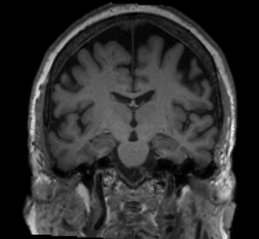
\includegraphics[height=6cm]{Figures/Brain__1.CN.png}
      \captionof{figure}{Normal}
    \end{minipage}%
    \hfill
    %================================
    \begin{minipage}{.32\linewidth}
      \centering
      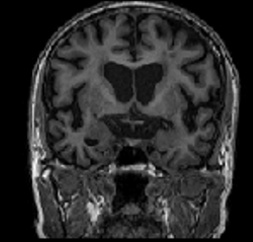
\includegraphics[height=6cm]{Figures/Brain__3.AD.png}
      \captionof{figure}{Alzheimer's Disease}
    \end{minipage}
    \hfill
    %================================
    \begin{minipage}{.32\linewidth}
      \centering
      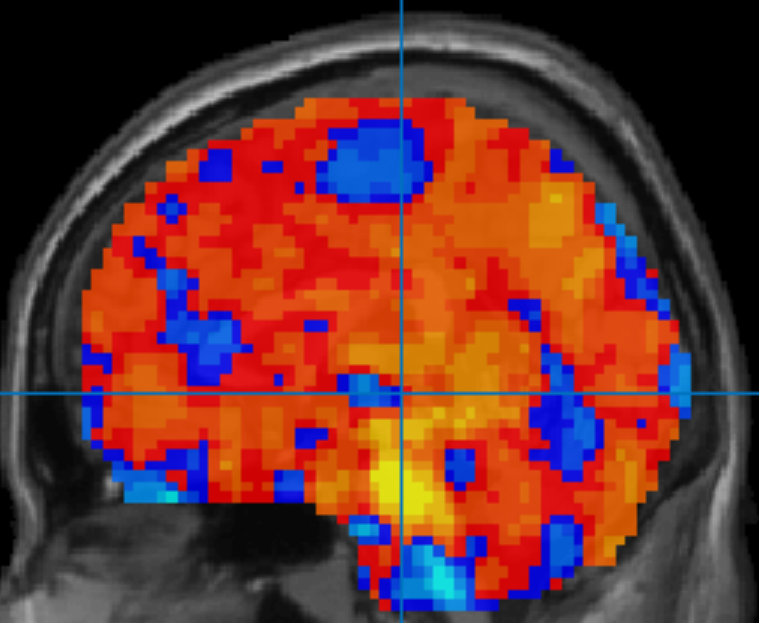
\includegraphics[height=6cm]{Figures/FC_Sagittal.png}
      \captionof{figure}{Functional Activity}
    \end{minipage}
\end{tikzfigure}




    
  %   \begin{tikzfigure}
  %       \centering
  %       \begin{minipage}{.50\linewidth}
  %         \centering
  %         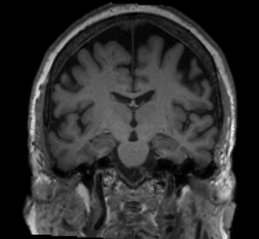
\includegraphics[height=9cm]{Figures/Brain__1.CN.png}
  %         \caption{\textcolor{col_CN}{CN}}
  %       \end{minipage}%
  %       \hfill
  %       \begin{minipage}{.50\linewidth}
  %         \centering
  %         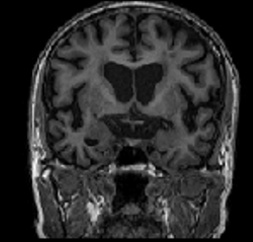
\includegraphics[height=9cm]{Figures/Brain__3.AD.png}
  %         \caption{\textcolor{col_AD}{Dementia}}
  %       \end{minipage}
  %   \end{tikzfigure}
    
    \begin{itemize}
        % \item Dementia shows 3 progressive stages.     
        \item \small Alzheimer's Disease (AD) is incurable.

        \item \small  Different \textbf{brain atrophy} can be seen between AD and normal patients.

        \item \small  By monitoring and identifying related brain regions that are characteristic of AD, researchers can better understand the progression of the disease, leading to the development of more effective interventions.
        
        \item \small  Hence, their \textbf{functional activity} in Resting-State fMRI (RS-fMRI) should be different. 

        \item \small From RS-fMRI, we can obtain \textbf{blood-oxygen-level-dependent (BOLD) times courses} for each region of interest (ROI) on brains.

    \end{itemize}
% \noindent
